% !TeX root = ../thuthesis-example.tex

\chapter{Conclusion and Future Work}

\section{Future directions}

A possible NUIX-Studio development timeline was created.

As seen in Figure~\ref{fig:Timeline-figure}, the development started with providing support for Virtual reality headsets. The next step was implementing openHAB and database support to perform simultaneous interaction in the same environment across several App instances. However, the Things designer is not fully developed since further research is needed to provide a wider variety of supported Widgets and Items.

\begin{figure}
  \centering
  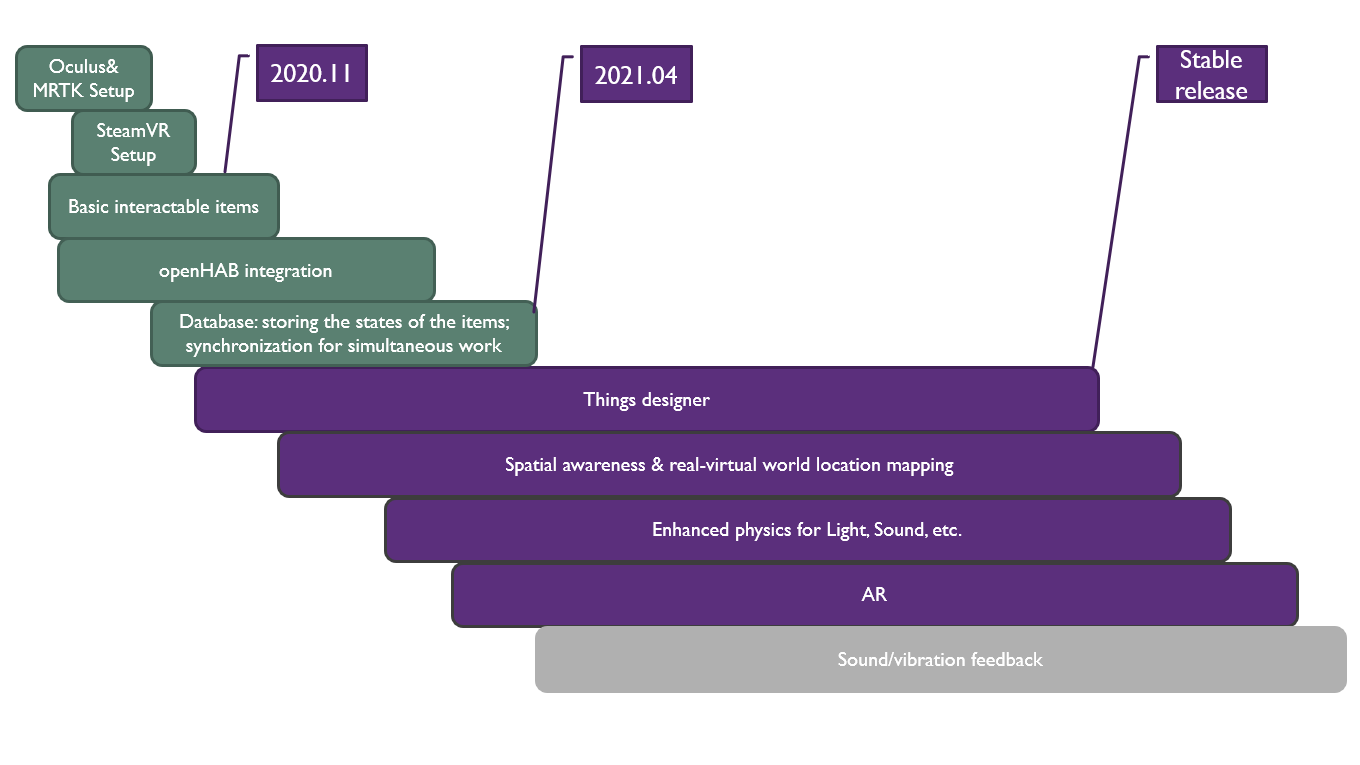
\includegraphics[width=0.9\linewidth]{figures/Timeline.png}
  \caption{Timeline for NUIX-Studio platform development. Green indicates that the task has been developed, blue indicates that the task development has been started, and grey indicates that it has not yet been started.}
  \label{fig:Timeline-figure}
\end{figure}

The Mixed Reality toolkit can provide real-world environmental awareness for apps running on Hololens. It is already possible to run the NUIX-Studio App on Hololens, although it has not been tested yet. Using spatial awareness, the NUIX-Studio App will be able to align virtual Widgets onto IoT devices. Developing real-virtual world location mapping for the Widgets in Virtual reality will be required as well.

Currently, only advanced illumination can be computed on the NUIX-Studio APP. Researchers may need more accurate data to create new IoT devices. In this case, Unity Game Engine can be extended with more precise light, sound, and other physics support.

Enabling AR support requires adding new interaction techniques and training Deep learning models to provide object recognition. Users can use both AR and VR to research new IoT devices, with AR being responsible for retrieving the coordinates of the devices from the real world (by OpenCV, Tensoflow Graphics, etc.), and VR for visualizing environments that are difficult or impossible to implement in AR (for example, flying on a plane or driving a car).

Augmented reality, Virtual reality, and Mixed Reality are not the only interfaces to interact with IoT in the virtual world. What if the feedback from IoT devices is provided only by sound and vibrations? The NUIX-Studio can be adapted for such limitations. One of the example uses of this approach is research for visually impaired people in an IoT environment.

During the whole development cycle, the NUIX-Studio API must be up-to-date for use in external projects. 

\section{Summary}


The result of the research is a developed concept of the platform, as well as the basis for further development of tools for creating IoT devices in Virtual, Augmented and Mixed reality. By creating a prototype platform, the following hypothesis have been proven:

\begin{enumerate}
    \item  Using the presented architecture, any IoT device can be added to the virtual world;
    \item It is possible to add new functionality to existing IoT devices inside the VR environment;
    \item It is possible to create completely virtual devices and embed them in the same environment with real devices;
    \item The synchronization time between devices within the IoT-VR environment is currently limited by the network speed;
    \item It is possible for several users to work simultaneously in one IoT-VR environment;
    \item To improve user experience, it is necessary to separate data and interaction calculation tasks between different application instances;
    \item The platform is scalable;
\end{enumerate}


The developed solution has the following advantages:\footnote{Considering that there are no similar solutions on the market, these advantages can be considered a reserve for the future}
\begin{enumerate}
    \item Integration of third-party solutions is possible both from the IoT support side and from the VR side;
    \item The platform's implementation is lightweight and is not based on many third-party frameworks;
    \item The development team can add new members without the need to teach people new technologies since the main part of the platform is written in C\# inside the Unity engine. It also has the advantage of more conveniently adding external projects into the platform;
    \item Researchers can use the platform API to create elements of interaction with IoT devices;
    \item A tool called Thing designer allows researchers to create new IoT devices using both VR and the Web interface;
    \item A tool is being developed to track the position of real devices and synchronize with their position in the virtual world (can start from using QR-codes);
    \item It is shown that the platform is capable of working not only with Virtual but also with Augmented and Mixed reality, and simultaneous operation of each reality-based App within the same IoT environment is possible;
    \item It is shown that the platform provides support for complex physical computations.
\end{enumerate}

Nevertheless, there are still limitations associated with creating a complete copy of the real-world environment inside the virtual one, particularly surrounding the need to manually add movable objects in the form of Items and Widgets.

The author hopes that this research will form the basis of a product that will have a significant value in the future, allowing the creation of new devices, including those for use in new generation networks.